%Etude des solutions de réalisation technique possible
%Choix technologique retenus
%Justification de ces choix avec avantages et inconvénients

Pour notre commanditaire, il est également essentiel que l'ensemble du projet et les outils utilisés soient open source.
Cette contrainte a été respectée, et nous n'avons donc pas jugé utile de préciser que tous les outils suivants sont open source.

\subsection{Extraction du transcript}
Afin d'analyser un document pdf, nous devons en premier lieux en extraire le texte brut, appelé ici \textit{transcript}.
L'extraction du transcript dépend de la manière dont le document a été enregistré : Souvent le texte est directement présent dans le document lui même, mais il arrive que le pdf soit stocké sous la forme d'une suite d'images (lorsque le document est un scan par exemple).

\subsubsection {Cas du pdf \textit{full text}}
Le format pdf contient normalement directement le transcript du document.
Dans ce cas, plusieurs méthodes très simples existent pour le récupérer : pdftotext, poppler, \ldots 
Nous avons choisis pdftotext car c'est l'outil open source le plus suivi et le plus utilisé, ce qui le rend très probable d'être déjà présent.
De plus sa popularité le rend très probablement plus durable.

\subsubsection {Cas du pdf image}
Si le document pdf ne contient pas de texte, nous devons passer par des techniques d'OCR (Optical Character Recognition).
Ces techniques nous permettent d'extraire le texte d'une image grâce a des techniques avancées de machine learning.

Nos recherches pour l'état de l'art a relevé les techniques suivantes :
\begin {itemize}
\item Tesseract : État de l'art de l'OCR open source pour le moment (score d'environ 90\%)
\item OCRupus : Logiciel très réputé d'OCR (score d'environ 70\%)
\end {itemize}
Nous avons écarté l'idée de construire notre propre modèle au vu du temps très limité du projet.
Notre choix s'est porté sur l'état de l'art actuel, Tesseract, pour ses plus grandes performances et le fait qu'une librairie python est disponible pour l'utiliser directement.

Les logiciels d'OCR peuvent être utilisés directement sur les documents pdf transformés en images mais les performances obtenues ne seront pas optimales.
Le document traité doit passer par une étape de traitement d'image, puis de nettoyage du texte obtenu, qui contient de nombreuses erreurs.

\subsection{Extraction de la taxonomie}
%inventaire des méthodes d'extraction de taxonomie 
La taxonomie est un arbre fixe de termes fermés permettant de classer un document par termes représentants un contexte.
La classification du document dans une taxonomie permet par la suite d'affiner considérablement la recherche et le regroupement d'un document par catégories.

\subsubsection{Apprentissage supervisé}
L'association d'un document a un ensemble fermé de termes oriente naturellement vers l'utilisation d'un apprentissage supervisé.
En utilisant un modèle d'apprentissage profond, nous pourrions faire en sorte d'apprendre a associer une ou plusieurs taxonomie a un document, \textit{via} un \textit{embedding}, comme doc2vec\cite{doc2vec}.
Malheureusement des systèmes de ce type sont immédiatement exclus pour plusieurs raisons.
Tout d'abord ce système n'est pas adapté pour générer la grande quantité de taxonomies possibles pour un document, et est plutôt utilisable pour quelques taxonomies précises.
Mais la limitation principale est qu'il n'existe pas de corpus de documents annotés, ce qui rend l'utilisation de l'apprentissage supervisé impossible.

Le temps étant une ressource précieuse dans ce projet, nous ne pouvions nous attarder sur la création d'un tel corpus.

\subsubsection{Apprentissage non supervisé}
L'absence de base de donnée oriente le choix de la méthode vers la classification non supervisé.
Cependant les techniques de ce domaine sont difficilement adaptables a notre sujet: l'apprentissage non supervisé regroupe les documents dans des classes uniques non définies.
Ces classes sont déduites par le modèle lui même, et ne sont donc pas taxonomiques.
De plus le fait que la classe de sortie d'un document soit unique ne permet pas d'obtenir plusieurs taxonomies.

Nous pouvons cependant imaginer une donnée de classement documentaire sous la forme d'un regroupement par apprentissage non supervisé pour retrouver des documents semblables.


\subsubsection{Word2vec}
Le but du module taxonomique étant d'associer a des documents des mots provenant d'un ensemble de termes fermé, nous avons étudié la possibilité d'utiliser un word2vec\cite{word2vec} ou un doc2vec de façon non supervisé (en raison de l'absence de documents labellisées).

L'idée générale de word2vec et de doc2vec est d'associer a un mot ou a un paragraphe/document un vecteur numérique de taille fixe, généralement avec une centaine de dimensions.
Cette association, ou \textit{embedding}, est apprise du contexte du mot ou du document, c'est a dire des mots environnants.
En somme, des mots partageant le même contexte, e.g.\ parent/père auront des vecteurs qui seront proches selon une métrique choisie.
En général, nous utilisons la mesure de la similarité cosinus, donnée par la formule suivante:

\begin{equation}
	\text{similarité} = \frac{\vec{A} \dot \vec{B}}{\norm{\vec{A}}\norm{\vec{B}}}
	\label{eq:distCosine}
\end{equation}
où $A, B  \in \mathbb{R}^n$. Cette mesure renvoie un réel compris entre $[-1, 1]$

Cette mesure nous permet d'avoir une mesure de la similarité de deux mots ou groupes de mots.
Idéalement deux mots ayant un sens proche auront une mesure de la similarité cosinus proche de 1.
A l'inverse des mots ayant des sens opposés auront une mesure se rapprochant de -1. 

Nous voulions utiliser cette propriété pour obtenir des taxonomies a partir du texte du document.
En analysant chaque mot du document initial et en le passant par un word2vec, nous pouvions obtenir un \textit{embedding} du mot et le comparer avec la banque taxonomique, et donner au documents les mots de la taxonomie ayant une distance faible. 

\begin{figure}[h!]
  \centering
  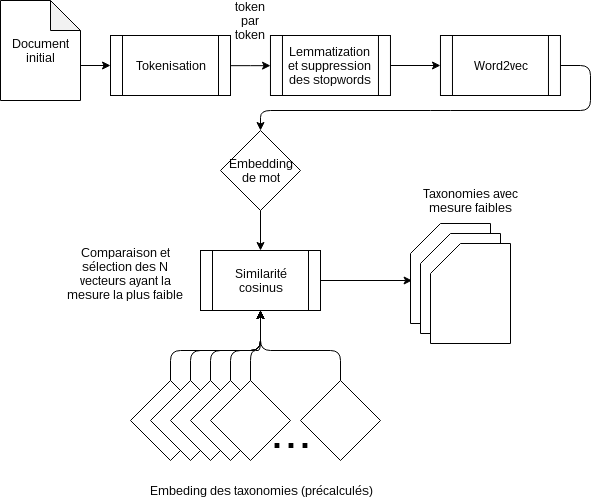
\includegraphics[width=0.8\textwidth]{taxoSchemaFoncInit.png}
	\caption[]{Schéma fonctionnel du module d'assignement taxonomique initial}
	\label{fig:taxoInit}
\end{figure}

\subsubsection{NLP}
L'utilisation des techniques du domaine du \textit{Natural Language Processing} permettent de traiter un texte pour en extraire des informations de plus haut niveau (le sens par exemple).
Le texte a analyser et la taxonomie peuvent être traités avec des méthodes de NLP afin de les normaliser et trouver les termes taxonomiques dont le sens se rapproche le plus de ce qu'on peut trouver dans le texte.

Il existe de très nombreuses méthodes de NLP utilisables pour cela, et nous avons choisis d'utiliser la lemmatization et la detection des mots d'importance.
La Lemmatization consiste a transformer un mot en sa racine, transformant par exemple `Nous sommes humains' deviendrait `nous être humain'.
La detection des mots d'importance nous permet d'enlever tous les mots de faible importance, et obtenir une phrase un peu plus propre.
Par exemple, `Délégation de signature' devient `Délégation signature'.


Nous avons choisi d'utiliser la méthode Word2vec, et la méthode NLP si word2vec ne fonctionnait pas, pour obtenir la taxonomie d'un document, les autres méthodes n'étant pas réalisables ou pas adaptées a notre problématique.
De plus word2vec et NLP peuvent être utilisées avec une autre taxonomie sans aucuns changements du code.
Cet élément est important car l'administration utilise plusieurs taxonomies. 


\subsection{Moteur de recherche}
Le moteur de recherche est la résultante visuelle de toutes les tâches techniques précédentes effectuées.
Après une étude de l’art, nous avons retenu Elasticsearch, état de l'art de la recherche open source.

Elasticsearch est moteur de recherche open source basé sous le logiciel Apache Lucene.
A l’aide d’un fichier JSON (JavaScript Object Notation) contenant les informations structurée extraites des documents, il indexe des documents via des requêtes HTTP\@.
Plusieurs sociétés, telles que Uber, Stack Overflow ou Udemy se basent sur ce système pour la recherche de produits/documents sur leurs sites. 
Cette approche nous permet de nous concentrer sur l'extraction des données plutôt que les problématiques d’indexations par score des documents.

\begin{figure}[h!]
  \centering
  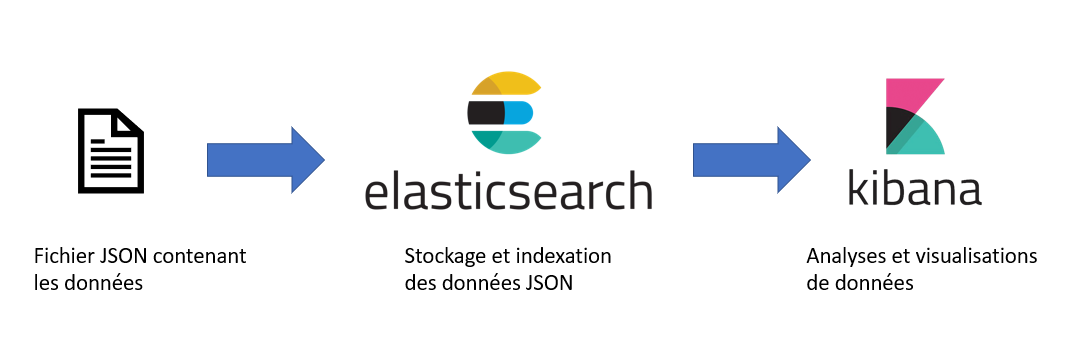
\includegraphics[width=0.8\textwidth]{ArchitectureElasticsearchKibana.PNG}
	\caption[]{Architecture Elasticsearch Kibana}
	\label{}
\end{figure}



\subsection{Interface du moteur de recherche}
Elasticsearch à lui tout seul ne suffit pas pour visualiser les données.
Comme dit précédemment, c’est à l’aide des requêtes HTTP que l’on peut effectuer une recherche.
Nous pouvons cependant utiliser des outils de visualisation interfacables avec Elasticsearch.

\subsubsection{Kibana}
Kibana est un greffon d'analyse de données pour ElasticSearch.
Il fournit plusieurs fonctions de visualisations qui permettent aux utilisateurs de créer des représentations visuelles (diagrammes barres/ligne, nuages de points, \ldots) pour représenter les informations de recherche Elasticsearch.

\begin{figure}[h!]
  \centering
  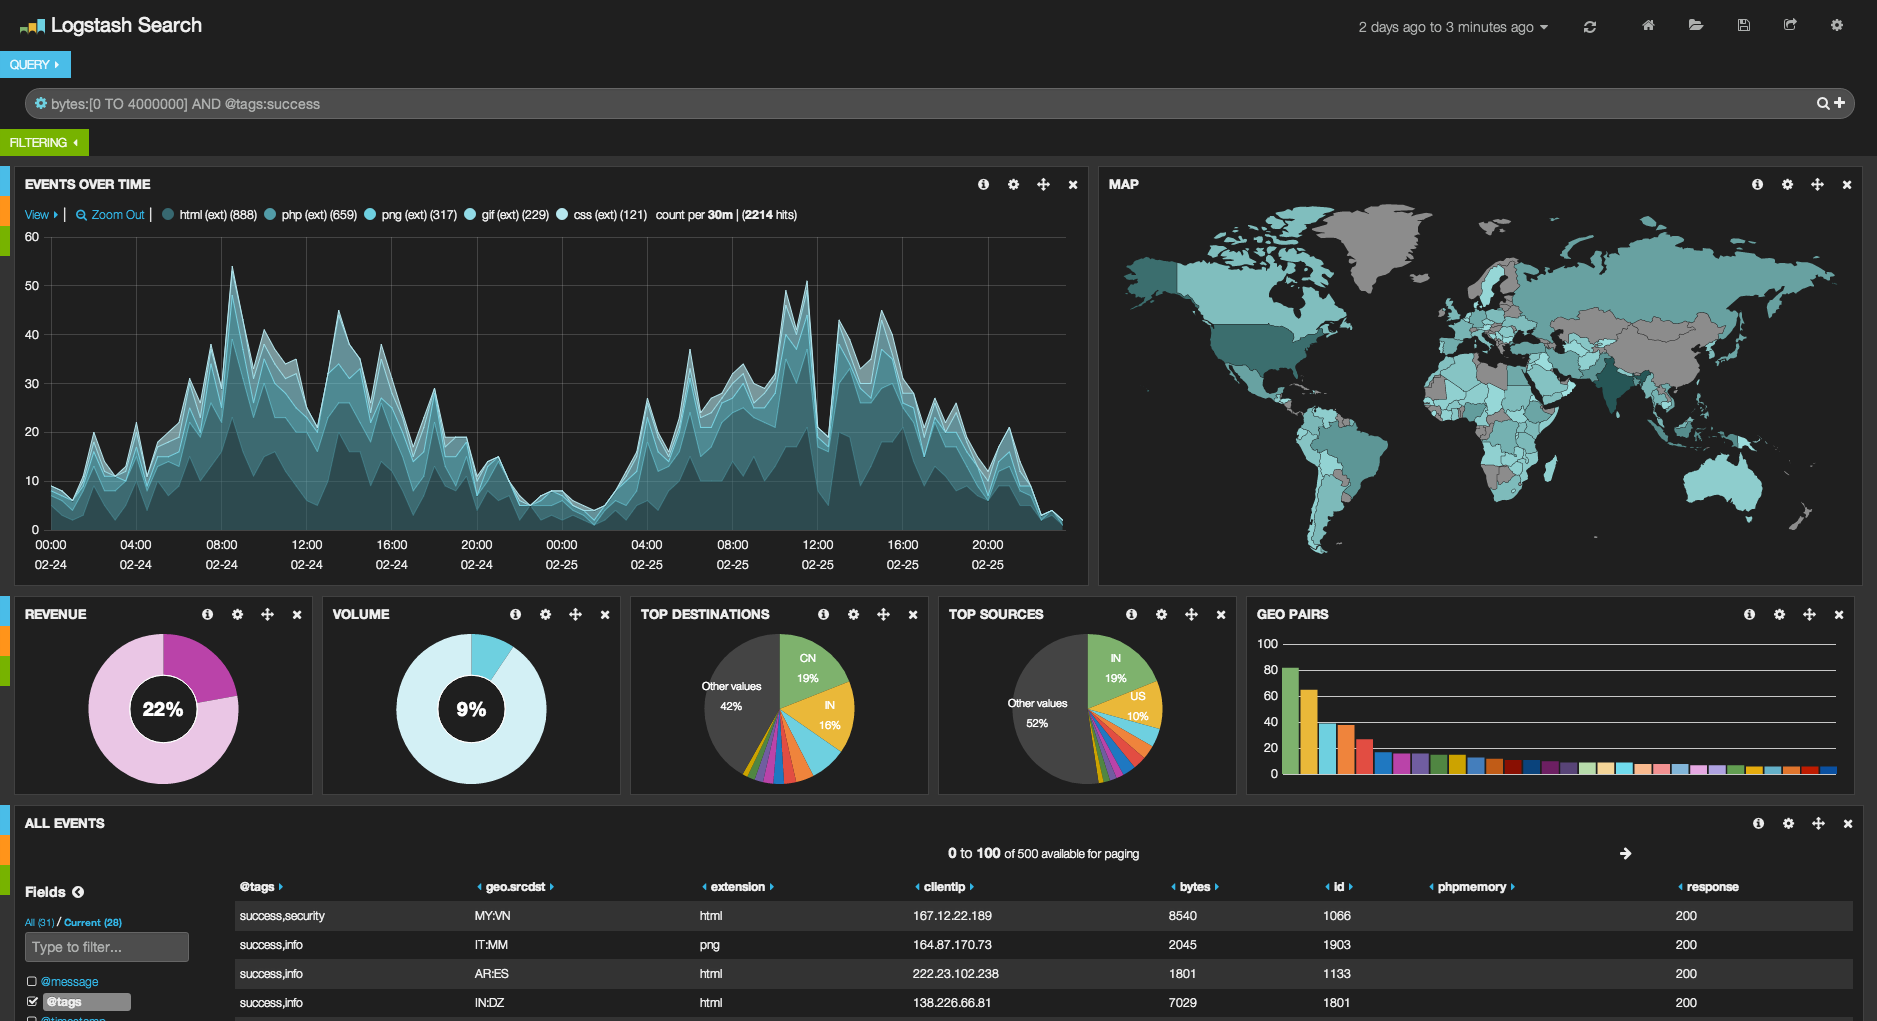
\includegraphics[width=0.8\textwidth]{visualisationKibana.png}
	\caption[]{Exemple de visualisation des données JSON sur Kibana}
	\label{}
\end{figure}
Même si pour un PoC, cela est présentable, Kibana est loin d’être ergonomique.

Le couple Elasticsearch/Kibana permet de construire un moteur de recherche basique présentant une visualisation technique des données.
Cependant, cette approche est très orientée analyse de données, et il ne faut pas qu'une contrainte du PoC est qu'il doit être \textit{user-friendly}.
Premièrement, l’utilisateur doit spécifier son champ de recherche en écrivant fields.champ afin d’effectuer une recherche.
Sachant que l’utilisation du moteur de recherche sera effectuée par plusieurs personnes de la préfecture non qualifiés techniquement, il serait préférable qu'il soit simple d’utilisation.
De plus, les fonctionnalités de Kibana qui sont orientés analyse de données, ce qui n'est pas notre sujet principal.

\begin{itemize}
    \item Avantages 
        \begin{itemize}
            \item Indexation directe avec Elasticsearch
            \item Visualisation des données avec Kibana
        \end{itemize}
    \item Inconvénient 
        \begin{itemize}
        \item Orienté analyse de données avec Kibana
        \end{itemize}
\end{itemize}


\subsubsection{Reactivesearch/Appbase.io}
Reactivesearch comme son nom l’indique se compose de React associé a Elasticsearch.

React aussi appelé React.js ou ReactJS est une bibliothèque JavaScript développée par Facebook en 2013.
Le but principal de cette bibliothèque est de faciliter la création d’application web mono page, en mettant des composants a disposition de l'utilisateur pour générer une page (ou portion) HTML lors d'un changement d'état.

Plusieurs sociétés telles que Facebook, Netflix, Yahoo ou WhatsApp l’utilisent.
Son avantage est que sa facilité d'utilisation et de développement, certains outils graphiques permettent de créer une page web en moins d'une heure.

Utiliser le site \href{https://appbase.io/}{appbase.io} pour programmer avec Reactivesearch est très intuitif.
Ce site permet d’importer des données au format JSON et d'obtenir directement un template de site mono page\@.

De plus, Reactivesearch est relié a des outils d'analyse et de statistiques des recherches effectuées par les utilisateurs.
Appbase se compose d’un \textit{Daily search volume} listant l’historique des recherches effectuées sur notre page Reactivesearch. 

Lors de l’import des données JSON, un ID personnel est envoyé, et permet aux possesseurs de l'ID d’accéder au JSON\@.
De cette manière, seules les personnes en possession de l'ID peuvent accéder et développer une page web avec les données du JSON importé. 

\begin{figure}[h!]
  \centering
  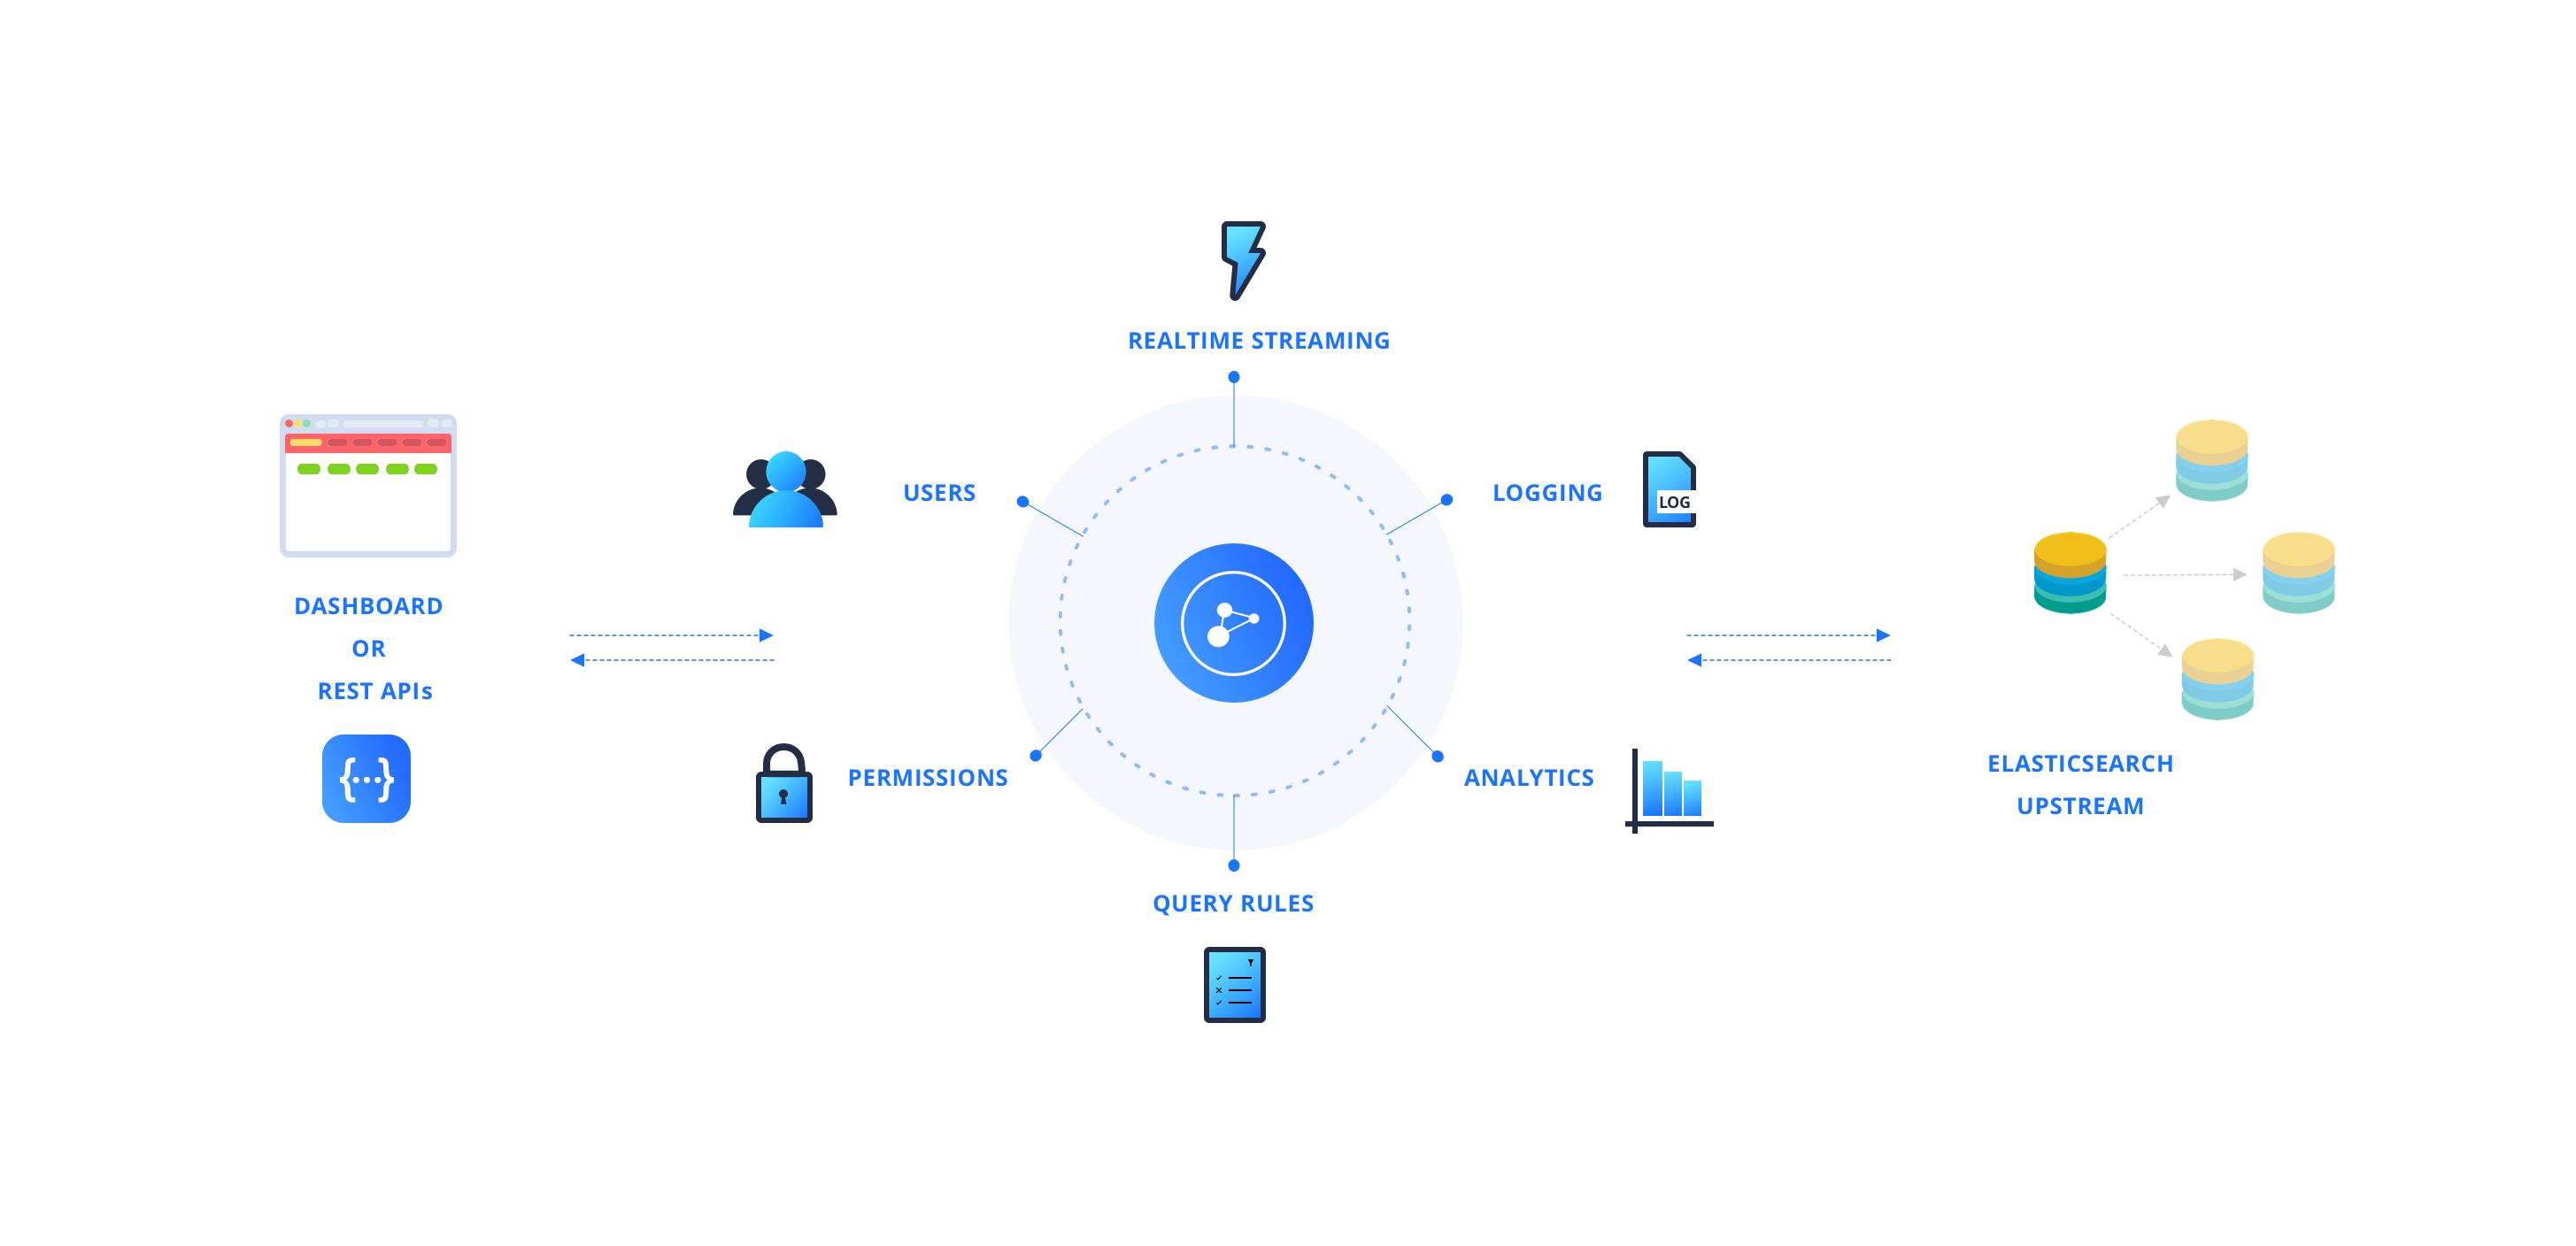
\includegraphics[width=\textwidth]{images/ArchitectureElasticsearchAppbase.png}
	\caption[]{Architecture Appbase.io et Elasticsearch}
	\label{archi_appbase}
\end{figure}

\newpage
\begin{itemize}
    \item Avantages 
        \begin{itemize}
            \item Indexation avec Elasticsearch
            \item Simple d’implémentation
            \item Sécurité relative d’accès aux données avec les credentials
            \item Analyse des historiques de recherche
            \item Mufti plateformes car en ligne
        \end{itemize}
    \item Inconvénients 
        \begin{itemize}
        \item Monopage (pas gênant pour notre application)
        \end{itemize}
\end{itemize}

Cette approche d’implémentation répond aux inconvénients de la visualisation avec Kibana.
Nous avons choisis donc choisis d'utiliser Reactivesearch pour les nombreux avantages par rapport a Kibana. 
